\subsection{CNV + RNA-seq}\label{sub:c_r_results}

\subsubsection{SDAE}

\begin{figure}[H]
     \centering
     \begin{subfigure}[b]{0.49\textwidth}
         \centering
         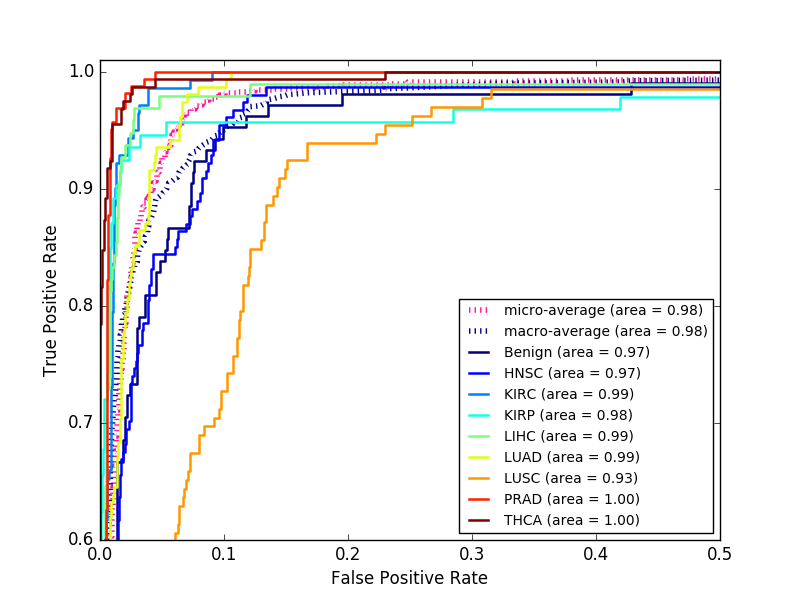
\includegraphics[width=\textwidth]{img/m_r/m_r_sdae_dgmu_roc.png}
         \caption{}
     \end{subfigure}
     \hfill
     \begin{subfigure}[b]{0.49\textwidth}
         \centering
         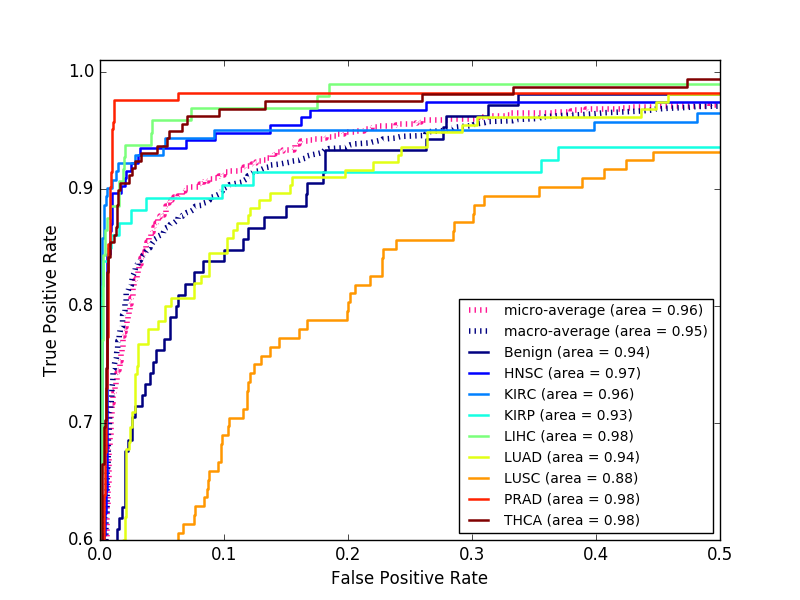
\includegraphics[width=\textwidth]{img/m_r/m_r_sdae_gmu_roc.png}
         \caption{}
     \end{subfigure}
     \hfill
     \begin{subfigure}[b]{0.49\textwidth}
         \centering
         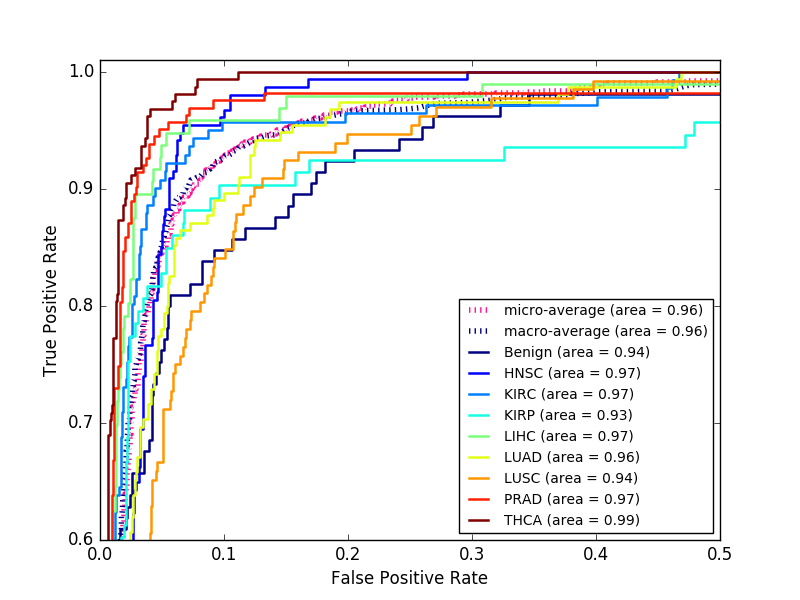
\includegraphics[width=\textwidth]{img/m_r/m_r_sdae_mlp_roc.png}
         \caption{}
     \end{subfigure}
     \begin{subfigure}[b]{0.49\textwidth}
         \centering
         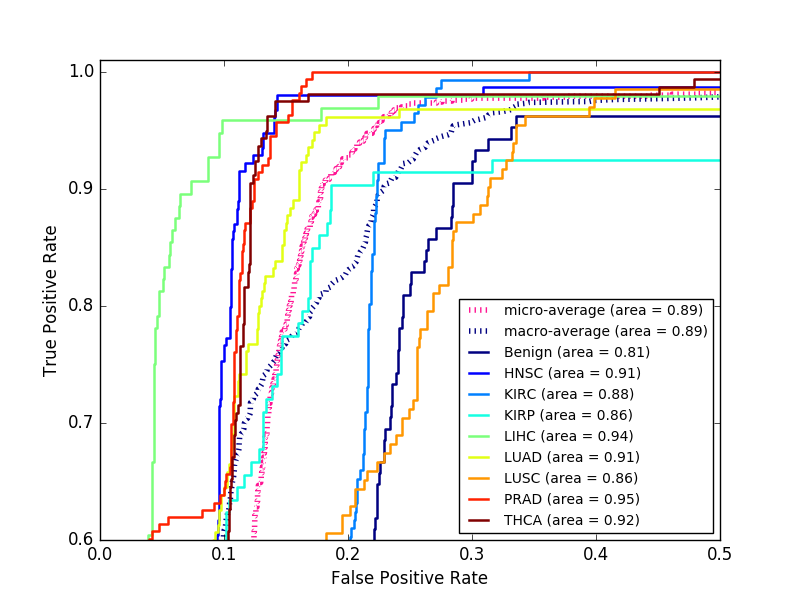
\includegraphics[width=\textwidth]{img/m_r/m_r_sdae_moe_roc.png}
         \caption{}
     \end{subfigure}
        \caption{miRNA-seq and RNA-seq SDAE bimodal model ROC plots for a) dGMU b) GMU c) MLP and d) ME.}
        \label{fig:m_r_sdae_roc}
\end{figure}

\begin{table}[H]
   \caption{Summary of classification agreement for miRNA-seq and RNA-seq SDAE reduced to 500 features.} 
   \small % text size of table content
   \centering % center the table
   \begin{tabular}{lllll} % alignment of each column data
   \toprule[\heavyrulewidth]\toprule[\heavyrulewidth]
   \textbf{Modality} & \textbf{Accuracy} & \textbf{Precision} & \textbf{Recall} & \textbf{F1-score} \\ 
   \midrule
   \multicolumn{1}{l}{\textbf{Bimodal}} \\
        dGMU & 0.9206 &	0.9218 & 0.9196	& 0.9207\\
        GMU  & 0.9123 &	0.9123 & 0.9123 & 0.9123\\
        MoE  & 0.8817 &	0.8813 & 0.8760 & 0.8786\\
        MLP  & 0.8829 &	0.8816 & 0.8750 & 0.8783\\
        SVM  & 0.8480 &	0.8444 & 0.8404 & 0.8424\\
   \midrule
   \multicolumn{1}{l}{\textbf{miRNA-seq}} \\
        MLP  & 0.8999 &	0.9020 & 0.8960 & 0.8990\\
        SVM  & 0.8673 &	0.8902 & 0.8592 & 0.8744\\
   \midrule
   \multicolumn{1}{l}{\textbf{RNA-seq}}  \\
        MLP  & 0.8361 &	0.6799 & 0.8379 & 0.8311\\
        SVM  & 0.8430 &	0.8381 & 0.8349 & 0.8365\\
   \bottomrule[\heavyrulewidth] 
   \end{tabular}
   \label{table:m_r_sdae_exp41}
\end{table}

\begin{figure}[H]
     \centering
     \begin{subfigure}[b]{\textwidth}
         \centering
         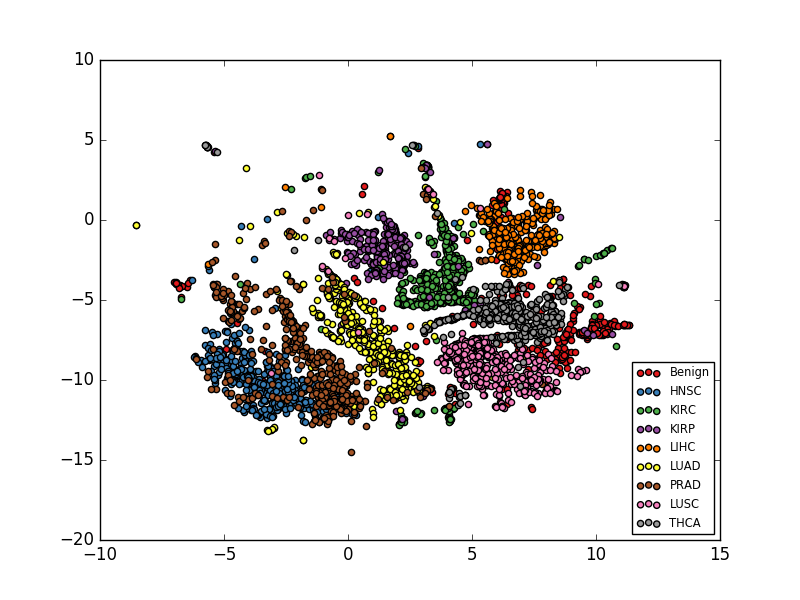
\includegraphics[width=\textwidth]{img/m_r/m_r_sdae_tsne.png}
     \end{subfigure}
        \caption{miRNA-seq and RNA-seq SDAE dGMU model latent space clustered with t-distributed stochastic neighbor embedding (t-SNE).}
        \label{fig:r_m_sdae_tsne}
\end{figure}

\subsubsection{DCF}

\begin{figure}[H]
     \centering
     \begin{subfigure}[b]{0.49\textwidth}
         \centering
         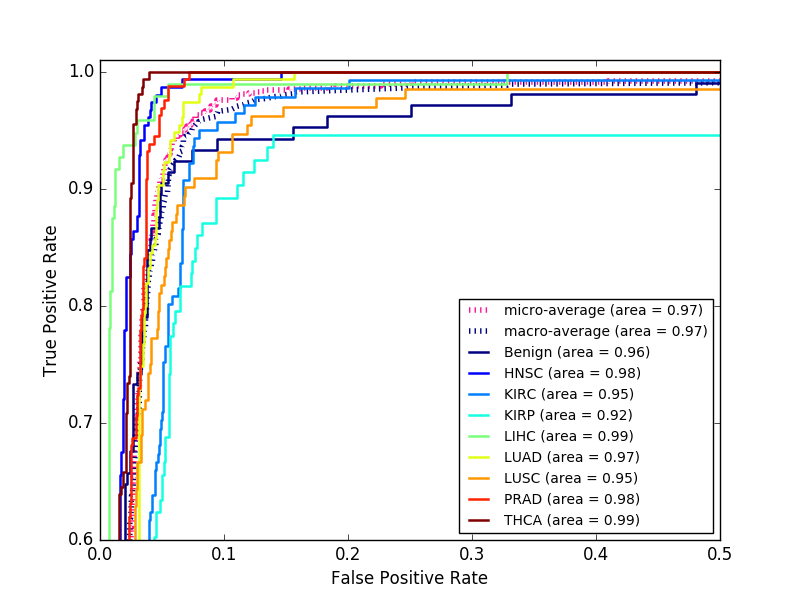
\includegraphics[width=\textwidth]{img/m_r/m_r_dcf_dgmu_roc.png}
         \caption{}
     \end{subfigure}
     \hfill
     \begin{subfigure}[b]{0.49\textwidth}
         \centering
         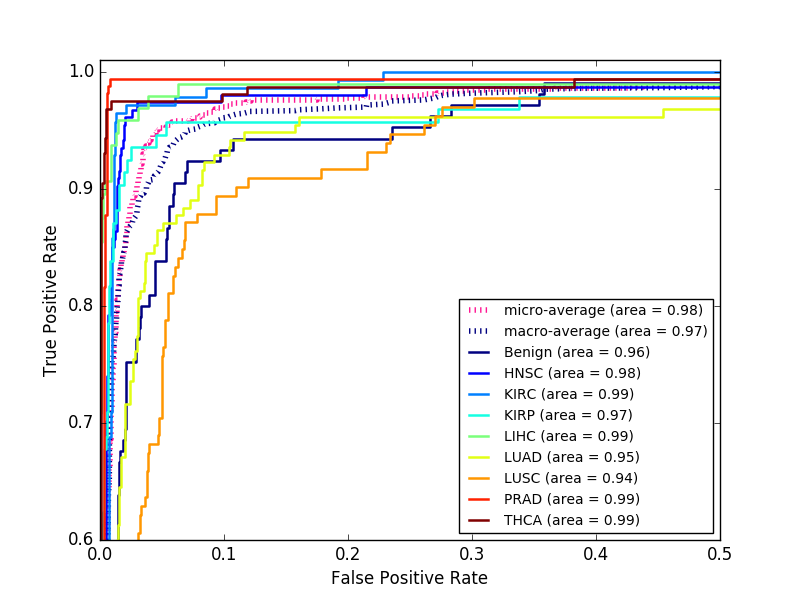
\includegraphics[width=\textwidth]{img/m_r/m_r_dcf_gmu_roc.png}
         \caption{}
     \end{subfigure}
     \hfill
     \begin{subfigure}[b]{0.49\textwidth}
         \centering
         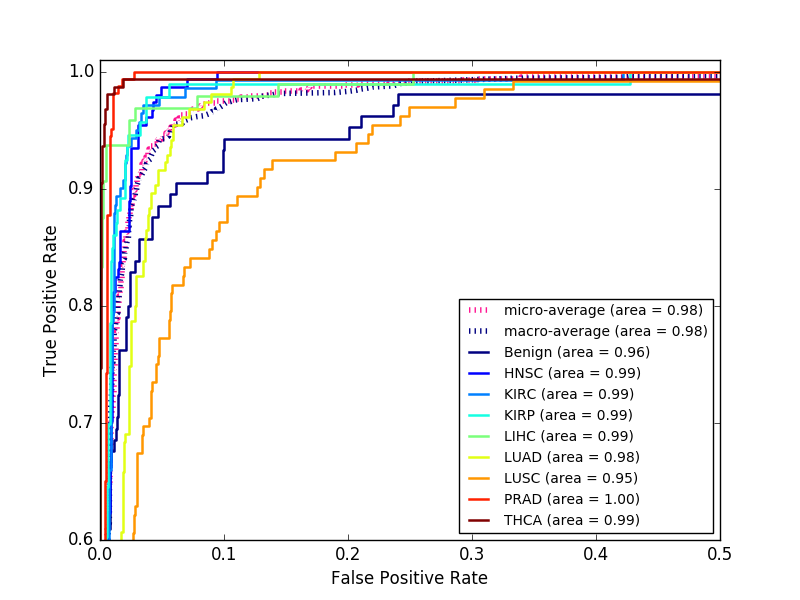
\includegraphics[width=\textwidth]{img/m_r/m_r_dcf_mlp_roc.png}
         \caption{}
     \end{subfigure}
     \begin{subfigure}[b]{0.49\textwidth}
         \centering
         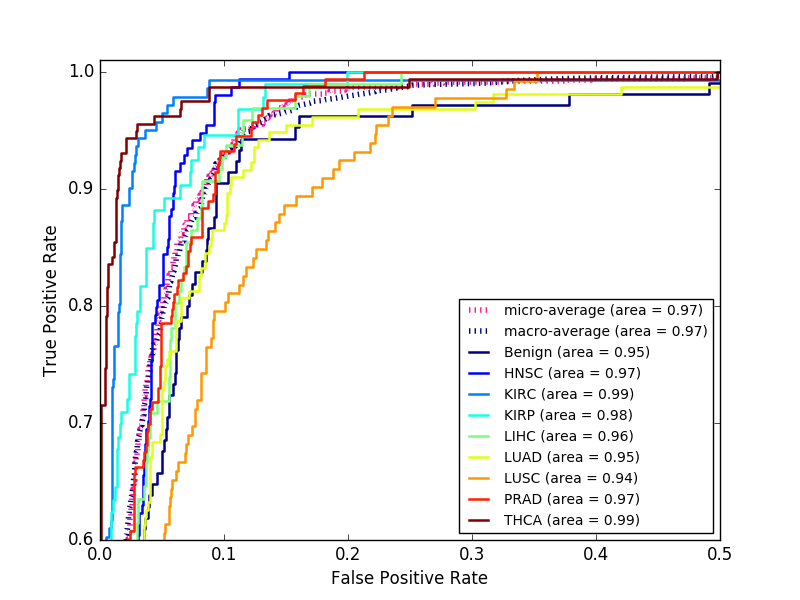
\includegraphics[width=\textwidth]{img/m_r/m_r_dcf_moe_roc.png}
         \caption{}
     \end{subfigure}
        \caption{miRNA-seq and RNA-seq DCF bimodal model ROC plots for a) dGMU b) GMU c) MLP and d) ME.}
        \label{fig:m_r_dcf_roc}
\end{figure}

\begin{table}[H]
   \caption{Summary of classification agreement for miRNA-seq and RNA-seq DCF reduced to 500 features.} 
   \small % text size of table content
   \centering % center the table
   \begin{tabular}{lllll} % alignment of each column data
   \toprule[\heavyrulewidth]\toprule[\heavyrulewidth]
   \textbf{Modality} & \textbf{Accuracy} & \textbf{Precision} & \textbf{Recall} & \textbf{F1-score} \\ 
   \midrule
   \multicolumn{1}{l}{\textbf{Bimodal}} \\
        dGMU & 0.9373 &	0.9385 & 0.9094 & 0.9362\\
        GMU  & 0.9332 &	0.9332 & 0.9332 & 0.9332\\
        MoE  & 0.9106 &	0.9120 & 0.9094 & 0.9107\\
        MLP  & 0.9215 &	0.9208 & 0.9136 & 0.9148\\
        SVM  & 0.8981 &	0.9081 & 0.8922 & 0.9001\\
   \midrule
   \multicolumn{1}{l}{\textbf{miRNA-seq}} \\
        MLP  & 0.8847 &	0.8881 & 0.8815 & 0.8848\\
        SVM  & 0.8739 &	0.8806 & 0.8690 & 0.8748\\
   \midrule
   \multicolumn{1}{l}{\textbf{RNA-seq}}  \\
        MLP  & 0.9023 &	0.9024 & 0.8940 & 0.8982\\
        SVM  & 0.9068 &	0.9116 & 0.9006 & 0.9061\\
   \bottomrule[\heavyrulewidth] 
   \end{tabular}
   \label{table:m_r_dcf_exp41}
\end{table}

\begin{figure}[H]
     \centering
     \begin{subfigure}[b]{\textwidth}
         \centering
         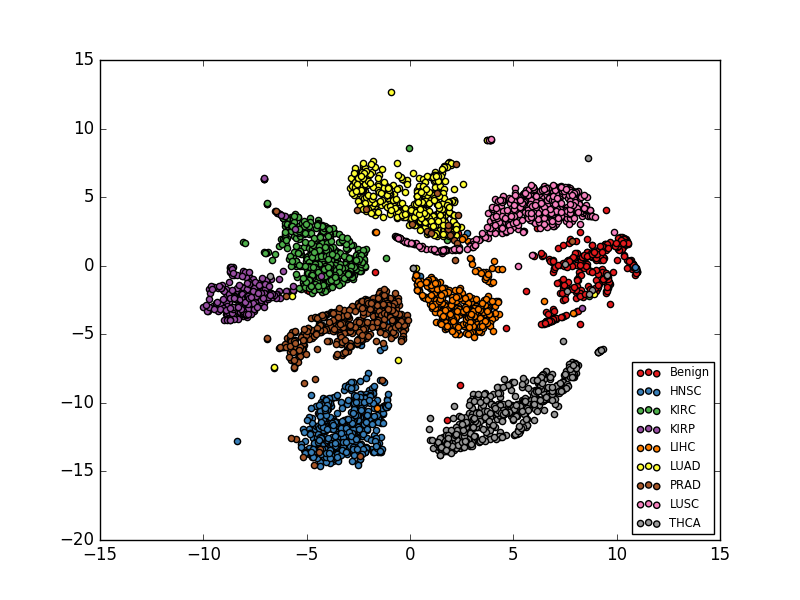
\includegraphics[width=\textwidth]{img/m_r/m_r_dcf_tsne.png}
     \end{subfigure}
        \caption{miRNA-seq and RNA-seq DCF dGMU model latent space clustered with t-distributed stochastic neighbor embedding (t-SNE).}
        \label{fig:r_m_dcf_tsne}
\end{figure}